%! Author = gramic
%! Date = 01.05.24

% Preamble
\begin{flushleft}
    \subsection{Technical Review der Umgebung}
    Die beiden Patroni-Nodes \texttt{sks1264} und \texttt{sks1265} sind Synchrone Replicas und der \texttt{sks1263} ist der Primary:
    \begin{figure}[H]
        \centering
        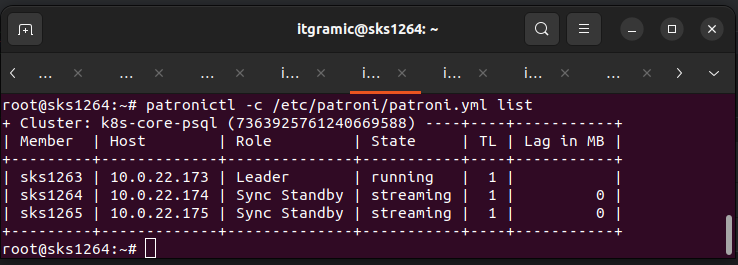
\includegraphics[width=1\linewidth]{source/implementation/construction_implementation/technical_review/patroni_list}
        \caption{Technical Review - Patroni Nodes}
        \label{fig:patroni_list}
    \end{figure}
\end{flushleft}
\begin{flushleft}
    Alle Datenbanken, die übergeben wurden, sind erstellt worden:
    \begin{figure}[H]
        \centering
        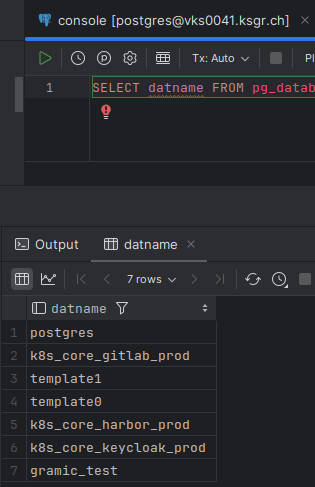
\includegraphics[width=0.5\linewidth]{source/implementation/construction_implementation/technical_review/datenbanken}
        \caption{Technical Review - Datenbanken}
        \label{fig:datenbanken}
    \end{figure}
\end{flushleft}
\begin{flushleft}
    Die Extensions wurden ebenfalls installiert:
    \begin{figure}[H]
        \centering
        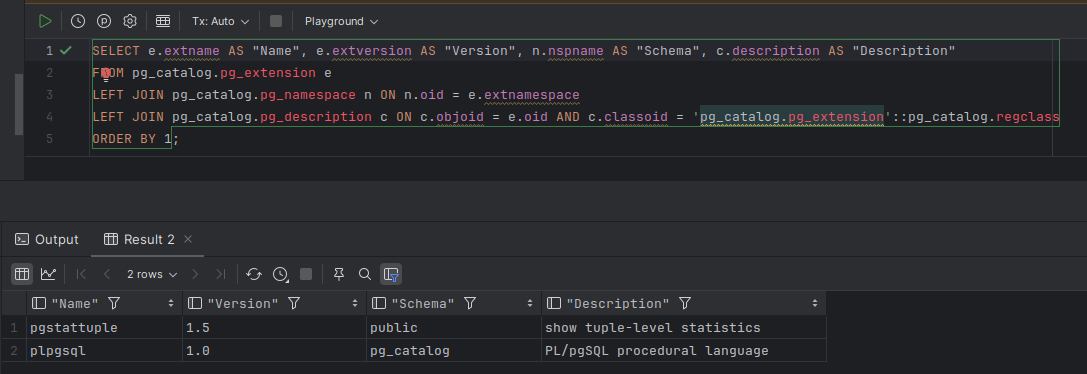
\includegraphics[width=1\linewidth]{source/implementation/construction_implementation/technical_review/extensions}
        \caption{Technical Review - PostgreSQL Extensions}
        \label{fig:extensions}
    \end{figure}
\end{flushleft}
\begin{flushleft}
    Die Rollen und User wurden erstellt:
    \begin{figure}[H]
        \centering
        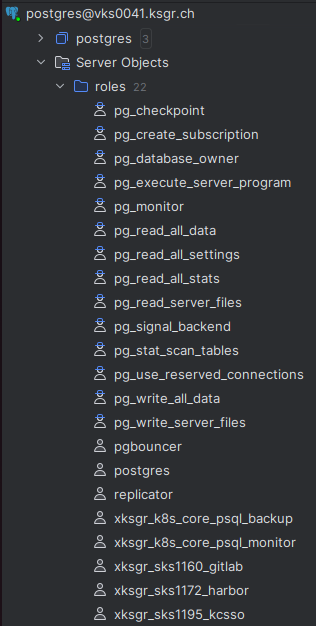
\includegraphics[width=0.5\linewidth]{source/implementation/construction_implementation/technical_review/user_roles}
        \caption{Technical Review - PostgreSQL User und Rollen}
        \label{fig:user_roles}
    \end{figure}
\end{flushleft}
\begin{flushleft}
    Die beiden HAproxy-Hosts \texttt{sks1266} und \texttt{sks1267} sind aktiv:
    \begin{figure}[H]
        \centering
        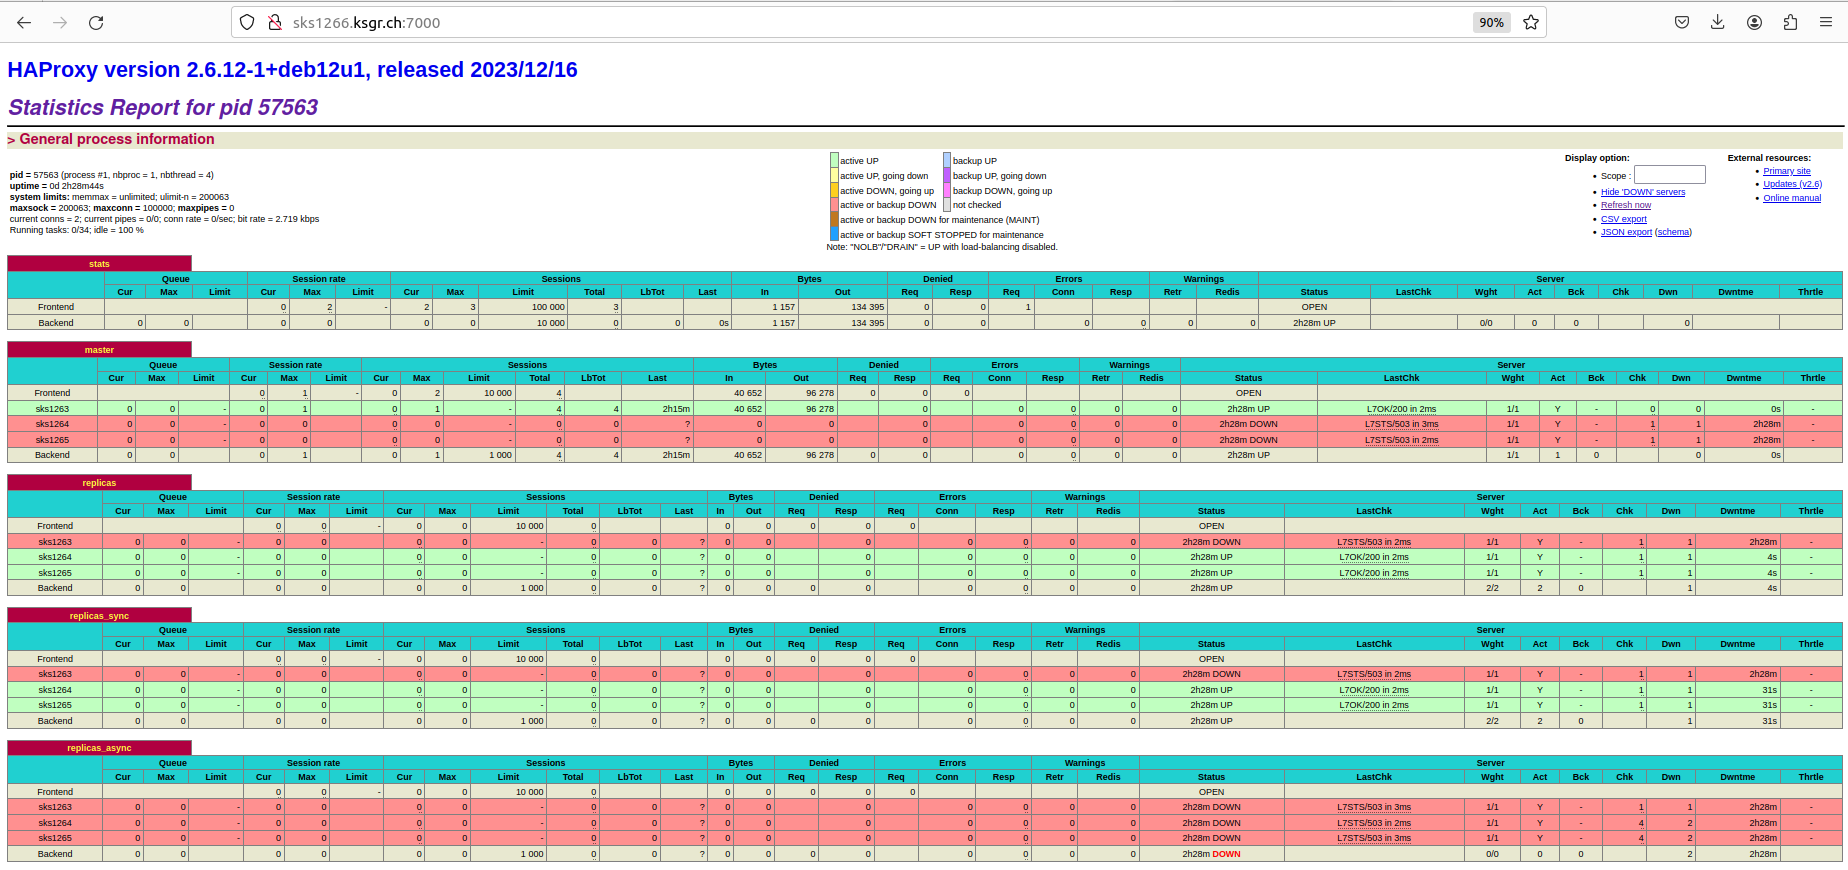
\includegraphics[width=1\linewidth]{source/implementation/construction_implementation/technical_review/haproxy_sks1266}
        \caption{Technical Review - HAproxy sks1266}
        \label{fig:haproxy_sks1266}
    \end{figure}
    \begin{figure}[H]
        \centering
        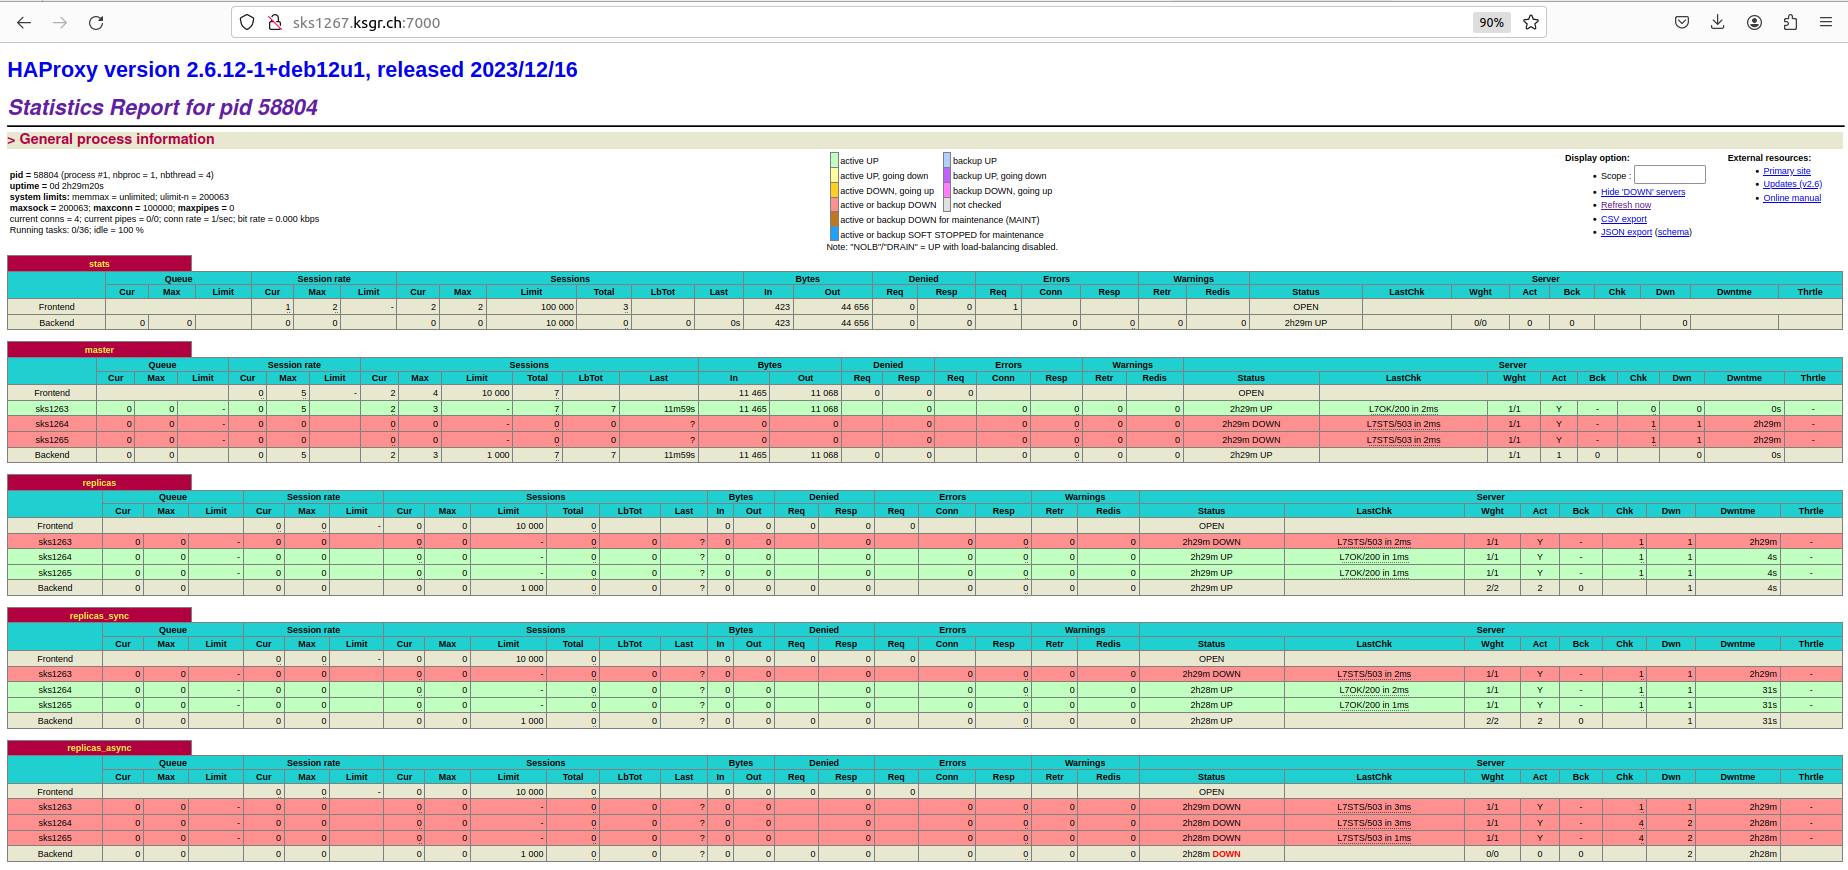
\includegraphics[width=1\linewidth]{source/implementation/construction_implementation/technical_review/haproxy_sks1267}
        \caption{Technical Review - HAproxy sks1267}
        \label{fig:haproxy_sks1267}
    \end{figure}
\end{flushleft}
\begin{flushleft}
    Die PgBouncer konfiguration passt.\\
    Alle via \Gls{Ansible} hinterlegten Datenbanken wurden erfasst:
    \begin{figure}[H]
        \centering
        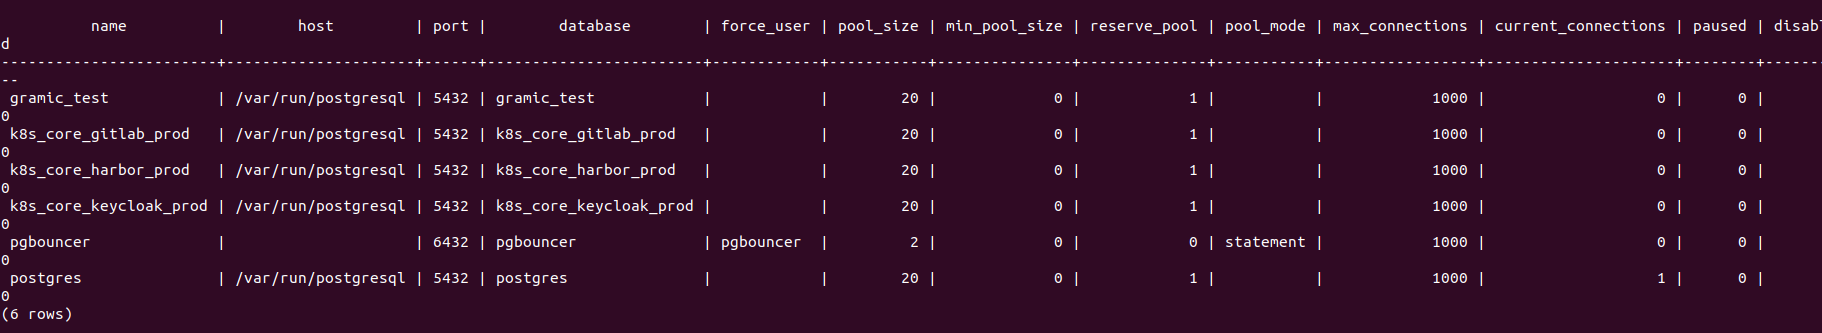
\includegraphics[width=1\linewidth]{source/implementation/construction_implementation/technical_review/pgbouncer_databases}
        \caption{Technical Review - PgBouncer - Datenbanken}
        \label{fig:pgbouncer_databases}
    \end{figure}
    Beim Auslesen der Stats und Datenbanken muss der richtige User gewählt werden.\\
    So hat der User \texttt{pgbouncer} keine Berechtigung, Lokal zuzugreifen.\\
    Auch nicht auf die Lokale Datenbank \texttt{pgbouncer}.\\
    Hierfür muss der User \texttt{postgres} verwendet werden:
\lstset{style=gra_codestyle}
\begin{lstlisting}[language=bash, caption=PgBouncer - Connect,captionpos=b,label={lst:pgbouncer_connect},breaklines=true]
psql -p 6432 -h 127.0.0.1 -U postgres -d pgbouncer
\end{lstlisting}
    Die Abfrage der Tabellen wird dann mittels folgendem Command gemacht:
\lstset{style=gra_codestyle}
\begin{lstlisting}[language=sql, caption=PgBouncer - Databases,captionpos=b,label={lst:pgbouncer_list_databases},breaklines=true]
show databases;
\end{lstlisting}
\end{flushleft}
\begin{flushleft}
    Die Logs werden einmal pro Tag neu erfasst:
    \begin{figure}[H]
        \centering
        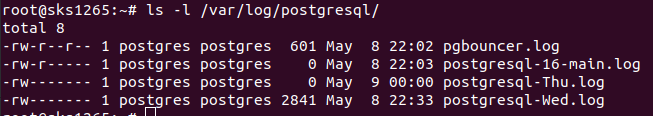
\includegraphics[width=1\linewidth]{source/implementation/construction_implementation/technical_review/postgresql_log_rotation}
        \caption{Technical Review - PostgreSQL - Log Rotation}
        \label{fig:postgresql_log_rotation}
    \end{figure}
    Die Einstellungen werden vorerst so belassen.\\
    Sobald dass \Gls{SIEM} betriebsbereit ist, wird das Format und die Frequenz entsprechend den Anforderungen angepasst.
\end{flushleft}